\section{Naravna in cela števila, izrazi, enačbe in neenačbe}

\begin{frame}
    \sectionpage
\end{frame}

\begin{frame}
    \tableofcontents[currentsection, hideothersubsections]
\end{frame}
        
    \subsection{Naravna in cela števila}

        \begin{frame}
            \frametitle{Naravna števila}

            \textbf{Množica naravnih števil}: 
                \begin{alertblock}{}
                    \centering\boldmath
                    $\mathbb{N}=\{1, 2, 3, 4, \ldots\}$
                \end{alertblock}

            Naravna števila so števila s katerimi štejemo.
            
            \medskip
            Naravna števila lahko predstavimo s \textbf{točko} na \textbf{številski premici}.
                \begin{figure}
                    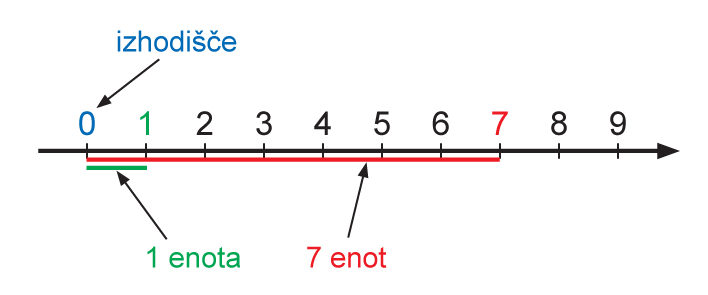
\includegraphics[scale=0.65]{Slike in skice/Stevilska_premica.png}
                \end{figure}
        \end{frame}

        \begin{frame}
            Množico naravnih števil definirajo \textbf{Peanovi aksiomi}:
            \begin{itemize}
                \item Vsako naravno število ($n$) ima svojega naslednika ($n+1$).
                \item Število $1$ ni naslednik nobenega naravnega števila.
                \item Različni naravni števili imata različna naslednika: ($n+1 \neq m+1;\quad n \neq m$).
                \item Če neka trditev velja za vsako naravno število in tudi za njegovega naslednika, velja za vsa naravna števila -- princip popolne indukcije.
            \end{itemize}
            
            \bigskip
            V množici $\mathbb{N}$ sta definirani notranji operaciji: \textbf{seštevanje} in \textbf{množenje}.
        \end{frame}

        \begin{frame}
            \textbf{\large{Seštevanje}}
            
            \bigskip
            Poljubnima naravnima številoma $a$ in $b$ priredimo \textbf{vsoto} $\mathbf{a+b}$.
            
            \bigskip
            Vsota naravnih števil je naravno število: $a, b \in \mathbb{N} \Rightarrow a+b \in \mathbb{N}$.
            
            \bigskip
            Lastnosti:
            \begin{itemize}
                \item \textit{\textbf{komutativnost}} členov/zakon o zamenjavi členov: $a+b = b+a$.
                \item \textit{\textbf{asociativnost}} členov/zakon o združevanju členov: $(a+b)+c = a+(b+c)$.
            \end{itemize}

        \end{frame}

        \begin{frame}
            \textbf{\large{Množenje}}
            
            \bigskip
            Poljubnima naravnima številoma $a$ in $b$ priredimo \textbf{produkt} $\mathbf{a\cdot b}$.
            
            \bigskip
            Produkt naravnih števil je naravno število: $a, b \in \mathbb{N} \Rightarrow a \cdot b \in \mathbb{N}$.            

            \bigskip
            Lastnosti:
            \begin{itemize}
                \item \textit{\textbf{komutativnost}} faktorjev/zakon o zamenjavi faktorjev: $a \cdot b = b \cdot a$.
                \item \textit{\textbf{asociativnost}} faktorjev/zakon o združevanju faktorjev: $(a \cdot b) \cdot c = a \cdot (b \cdot c)$.
                \item \textit{\textbf{distributivnost}}/zakon o razčlenjevanju: $a \cdot (b+c) = a \cdot b + a \cdot c$.
                \item zakon o nevtralnem elementu: $a \cdot 1 = a$.
            \end{itemize}

        \end{frame}

        \begin{frame}
            \frametitle{Cela števila}

            \textbf{Množica celih števil}: 
                \begin{alertblock}{}
                    \centering\boldmath
                    $\mathbb{Z} = \{\ldots, -2, -1, 0, 1, 2, 3, \ldots\}$
                \end{alertblock}

                Množica celih števil je definirana kot unija treh množic:
                $$\mathbb{Z} = \mathbb{Z}^- \cup \{0\} \cup \mathbb{Z}^+$$

                \begin{itemize}
                    \item množica \textbf{pozitivnih celih števil} ($\mathbb{Z}^+$) -- naravna števila;
                    \item \textbf{število 0};
                    \item množica \textbf{negativnih celih števil} ($\mathbb{Z}^-$) -- nasprotna števila vseh naravnih števil.
                \end{itemize}
                
                \medskip
                \textbf{Nasprotno število} števila $a$ je $-a$.
        \end{frame}

        \begin{frame}

            Poleg seštevanja in množenja je kot notranja operacija množice celih števil
            definirano še \textbf{odštevanje}.

            \bigskip
            \textbf{\large{Odštevanje}}
            
            \bigskip
            Poljubnima naravnima številoma $a$ in $b$ priredimo \textbf{razliko} $\mathbf{a - b}$.
            
            \bigskip
            Odštevanje definiramo kot prištevanje nasprotne vrednosti: $a-b = a+(-b)$

            \bigskip
            Za odštevanje velja zakon \textit{\textbf{distributivnosti}}: $a \cdot (b-c) = a \cdot b - a
            \cdot c$.

        \end{frame}

        \begin{frame}
            \textbf{\large{Računski zakoni}}

            \smallskip
            \begin{itemize}
                \item Komutativnostni zakon: $$a+b = b+a ~\text{in}~ a \cdot b = b \cdot a$$
                \item Asociativnostni zakon: $$a+(b+c) = (a+b)+c ~\text{in}~ a \cdot (b \cdot c) = (a \cdot b) \cdot c$$
                \item Zakon o nevtralnem elementu: $$a+0 = a ~\text{in}~ a \cdot 1 = a$$
                \item Zakon o inverznem/nasprotnem elementu: $$a+(-a) = 0$$
                \item Distributivnostni zakon: $$a \cdot (b \pm c) = a \cdot b \pm a \cdot c$$
            \end{itemize}


        \end{frame}

        \begin{frame}
            \textbf{\large{Pravila za računanje s celimi števili}}

            \bigskip
            \begin{itemize}
                \item $-(-a)=a$
                \item $0\cdot a=0$
                \item $-1 \cdot a =-a$
                \item $(-a)+(-b)=-(a+b)$
                \item $(-a)\cdot b=-(a\cdot b)=a\cdot (-b)$
                \item $(-a)\cdot(-b)=a\cdot b$
            \end{itemize}
        \end{frame}

        \begin{frame}

        \end{frame}


    \subsection{Računanje z naravnimi in celimi števili}

        \begin{frame}
            \frametitle{Računanje z naravnimi in celimi števili}
        \end{frame}

    \subsection{Izraz, enačba, neenačba}

        \begin{frame}
            \frametitle{Izraz, enačba, neenačba}
        \end{frame}

        % \begin{frame}
        %     \frametitle{Neenačba}

        %     \begin{alertblock}{Neenačba}
        %         Neenačba je zapis, v katerem sta dva izraza v ustrezni relaciji.

        %             $$\left\langle \textmd{izraz_1}\right\rangle < \left\langle \textmd{izraz_2}\right\rangle $$
        %             $$\left\langle \textmd{izraz_1}\right\rangle \leq \left\langle \textmd{izraz_2}\right\rangle $$ 
        %             $$\left\langle \textmd{izraz_1}\right\rangle > \left\langle \textmd{izraz_2}\right\rangle $$ 
        %             $$\left\langle \textmd{izraz_1}\right\rangle \geq \left\langle \textmd{izraz_2}\right\rangle $$  

        %     \end{alertblock}
        % \end{frame}

    \subsection{Računanje s potencami z naravnimi eksponenti}

        \begin{frame}
            \frametitle{Računanje s potencami z naravnimi eksponenti}

            Potenca $\mathbf{a^n}$, pri čemer je $n \in \mathbb{N}$, je produkt $n$ faktorjev enakih $a$.

            \begin{figure}
                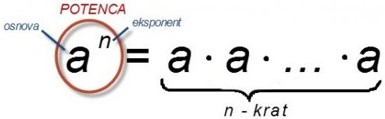
\includegraphics[scale=0.5]{Slike in skice/Potenca.jpg}
            \end{figure}
    
            \textbf{Pravila za računanje s potencami}:
            \begin{itemize}
                \item $\mathbf{a^n \cdot b^n = (ab)^n}$ - potenci z enakima eksponentoma zmnožimo tako, da zmnožimo osnovi in prepišemo eksponent
                \item $\mathbf{a^m \cdot a^n = a^{m+n}}$ - potenci z enako osnovo zmnožimo tako, da osnovo prepišemo in seštejemo eksponenta
                \item $\mathbf{(a^n)^m = a^{nm}}$ - potenco potenciramo tako, da osnovo prepišemo in zmnožimo eksponenta
            \end{itemize}

        \end{frame}

    \subsection{Razčlenjevanje izrazov}

        \begin{frame}
            \frametitle{Razčlenjevanje izrazov}
        \end{frame}

    \subsection{Razstavljanje izrazov v množici $\mathbb{Z}$}

        \begin{frame}
            \frametitle{Razstavljanje izrazov v množici $\mathbb{Z}$}
        \end{frame}

    \subsection{Reševanje linearnih in razcepnih enačb v množici $\mathbb{Z}$}

        \begin{frame}
            \frametitle{Reševanje linearnih in razcepnih enačb v množici $\mathbb{Z}$}
        \end{frame}

    \subsection{Reševanje linearnih neenačb v množici $\mathbb{Z}$}

        \begin{frame}
            \frametitle{Reševanje linearnih neenačb v množici $\mathbb{Z}$}
        \end{frame}
